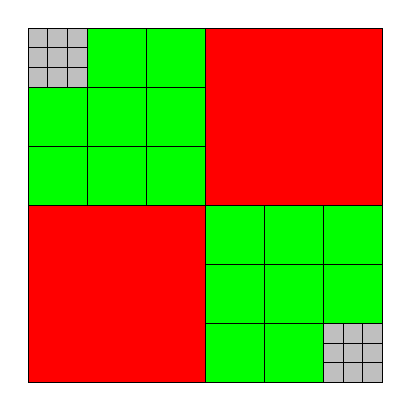
\begin{tikzpicture}[scale = 0.25]
    \def \Dx {12}
    \def \stp {1}
    \def \stpp {3}
  
      \def \za {0}
      % \def \zb {8}
      \def \zb {10}
      % \def \zc {16}
      \def \zc {20}
      \def \compx {18}
      \def \rx {3}
      \def \rxx {9}
      \def \nx {\compx/\rx}
      \def \nxx {\compx/\rxx}
  
    % style of grid
      \tikzset{nivelstyle1/.style={fill=green,opacity=1,very thin,line join=round}}
      \tikzset{nivelstyle2/.style={fill=red,opacity=1,very thin,line join=round}}
      \tikzset{nivelstyle0/.style={fill=lightgray,opacity=1,very thin,line join=round}}
  
      \draw[style=nivelstyle2] (0,0) rectangle (\compx,\compx);
      \draw[step=\rxx] (0,0) grid (\compx,\compx);
      \draw[style=nivelstyle1] (0,\compx/2) rectangle (\compx/2,\compx);
      \draw[step=\rx] (0,\compx/2) grid (\compx/2,\compx);
      \draw[style=nivelstyle1] (\compx/2,0) rectangle (\compx,\compx/2);
      \draw[step=\rx] (\compx/2,0) grid (\compx,\compx/2);
      \draw[style=nivelstyle0] (0,\compx) rectangle (\rx,\compx-\rx);
      \draw[step=1] (0,\compx) grid (\rx,\compx-\rx);
      \draw[style=nivelstyle0] (\compx-\rx,0) rectangle (\compx,\rx);
      \draw[step=1] (\compx-\rx,0) grid (\compx,\rx);
  
    % \draw[fill=red!80,draw=white] (\stp, \stp) rectangle (2*\stp, 2*\stp);
    % \draw[fill=red!80,draw=white] (4*\stp, \stp) rectangle (5*\stp, 2*\stp);
    % \draw[fill=red!80,draw=white] (7*\stp, \stp) rectangle (8*\stp, 2*\stp);
    % \draw[fill=red!80,draw=white] (10*\stp, \stp) rectangle (11*\stp, 2*\stp);
      %
    % \draw[fill=red!80,draw=white] (\stp, 4*\stp) rectangle (2*\stp, 5*\stp);
    % % \draw[fill=red!80,draw=white] (4*\stp, 4*\stp) rectangle (5*\stp, 5*\stp);
    % % \draw[fill=red!80,draw=white] (7*\stp, 4*\stp) rectangle (8*\stp, 5*\stp);
    % \draw[fill=red!80,draw=white] (10*\stp, 4*\stp) rectangle (11*\stp, 5*\stp);
      %
    % \draw[fill=red!80,draw=white] (\stp, 7*\stp) rectangle (2*\stp, 8*\stp);
    % \draw[fill=red!80,draw=white] (4*\stp, 7*\stp) rectangle (5*\stp, 8*\stp);
    % \draw[fill=red!80,draw=white] (7*\stp, 7*\stp) rectangle (8*\stp, 8*\stp);
    % \draw[fill=red!80,draw=white] (10*\stp, 7*\stp) rectangle (11*\stp, 8*\stp);
      %
    % \draw[fill=red!80,draw=white] (\stp, 10*\stp) rectangle (2*\stp, 11*\stp);
    % \draw[fill=red!80,draw=white] (4*\stp, 10*\stp) rectangle (5*\stp, 11*\stp);
    % \draw[fill=red!80,draw=white] (7*\stp, 10*\stp) rectangle (8*\stp, 11*\stp);
    % \draw[fill=red!80,draw=white] (10*\stp, 10*\stp) rectangle (11*\stp, 11*\stp);
      %
    % % \draw[fill=red!30,draw=white] (\stp*2,\stp*2) rectangle (\stp*3,\stp*3);
    % \draw[style=gridstyle1,step=\stp] (0,0) grid (\Dx,\Dx);
    % \draw[style=gridstyle2,step=\stpp] (0,0) grid (\Dx,\Dx);
      %
    % \draw[fill=lightgray!80,draw=black,opacity=0.6] (\stpp+\stp, \stpp+\stp) rectangle (2*\stpp+2*\stp, 2*\stpp+2*\stp);
    % \draw[fill=red!80,draw=none] (4*\stp, 4*\stp) rectangle (5*\stp, 5*\stp);
    % \draw[fill=red!80,draw=none] (7*\stp, 4*\stp) rectangle (8*\stp, 5*\stp);
    % \draw[fill=red!80,draw=none] (4*\stp, 7*\stp) rectangle (5*\stp, 8*\stp);
    % \draw[fill=red!80,draw=none] (7*\stp, 7*\stp) rectangle (8*\stp, 8*\stp);
    % \draw (2*\stpp+\stp/2,2*\stpp+\stp/2) node{$\voldual$};
  
    % \draw plot coordinates{(\stp*2+\stp/2,\stp*2+\stp/2)} node[sloped] {$\Omega_{i}$};
    % \draw[line width=2pt,color=blue] (\Dx/2, 0) -- (0,0) -- (0,\Dx) -- (\Dx/2,\Dx);
    % \draw[line width=2pt,color=red] (\Dx/2, 0) -- (\Dx,0) -- (\Dx,\Dx) -- (\Dx/2,\Dx);
    % \draw[->, ultra thick] (-2,\Dx/2+1) node[sloped, left]{$\Gamma_{D}$} -- (0,\Dx/2);
    % \draw[->, ultra thick] (\Dx+2,\Dx/2+1) node[sloped, right]{$\Gamma_{N}$} -- (\Dx,\Dx/2);
    % \draw[fill=yellow!50] (0.5,0.5) circle (0.2);
    % \draw plot [mark=*, mark size=2] coordinates{(0.5,0.5)};
    % \draw[fill=yellow!50] (\Dx-0.5,\Dx-0.5) circle (0.2);
    % \draw plot [mark=*, mark size=2] coordinates{(\Dx-0.5,\Dx-0.5)};
    % \draw[->, ultra thick] (-1,1) node[sloped, left]{$\Gamma_{I}$} -- (0.5,0.5);
    % \draw[->, ultra thick] (\Dx+0.5,\Dx+0.5) node[sloped, right]{$\Gamma_{P}$} -- (\Dx-0.5,\Dx-0.5);
    % \draw (\Dx/2,\Dx/2) node[sloped, above]{$\Omega$};
  \end{tikzpicture}
  